%!TEX root = ../../report.tex

\subsection{CityEngine \cite{Parish2001} \cite{Muller2006}}
\label{sub:cityengine}

CityEngine is a three-dimensional (3D) modeling software developed by Procedural Inc. (now part of the Esri R\&D Center). Specialized in the generation of 3D urban environments. With the procedural modeling approach, CityEngine enables the efficient creation of detailed and large-scale 3D city models with a lot of control from the user. This system applies the concept of Immediate Feedback by allowing the user to immediately see the results of each change. This is implemented through a set of sliders that are assigned to various indicators in the model that can be as high level as the \emph{size of the city} or as specific as the width of the windows or the number of floors in a building.

The following sections explain how CityEngine faces each of the steps in the generation of a city, such as road network generation or building modeling.

\begin{figure}[htbp]
  \centering
  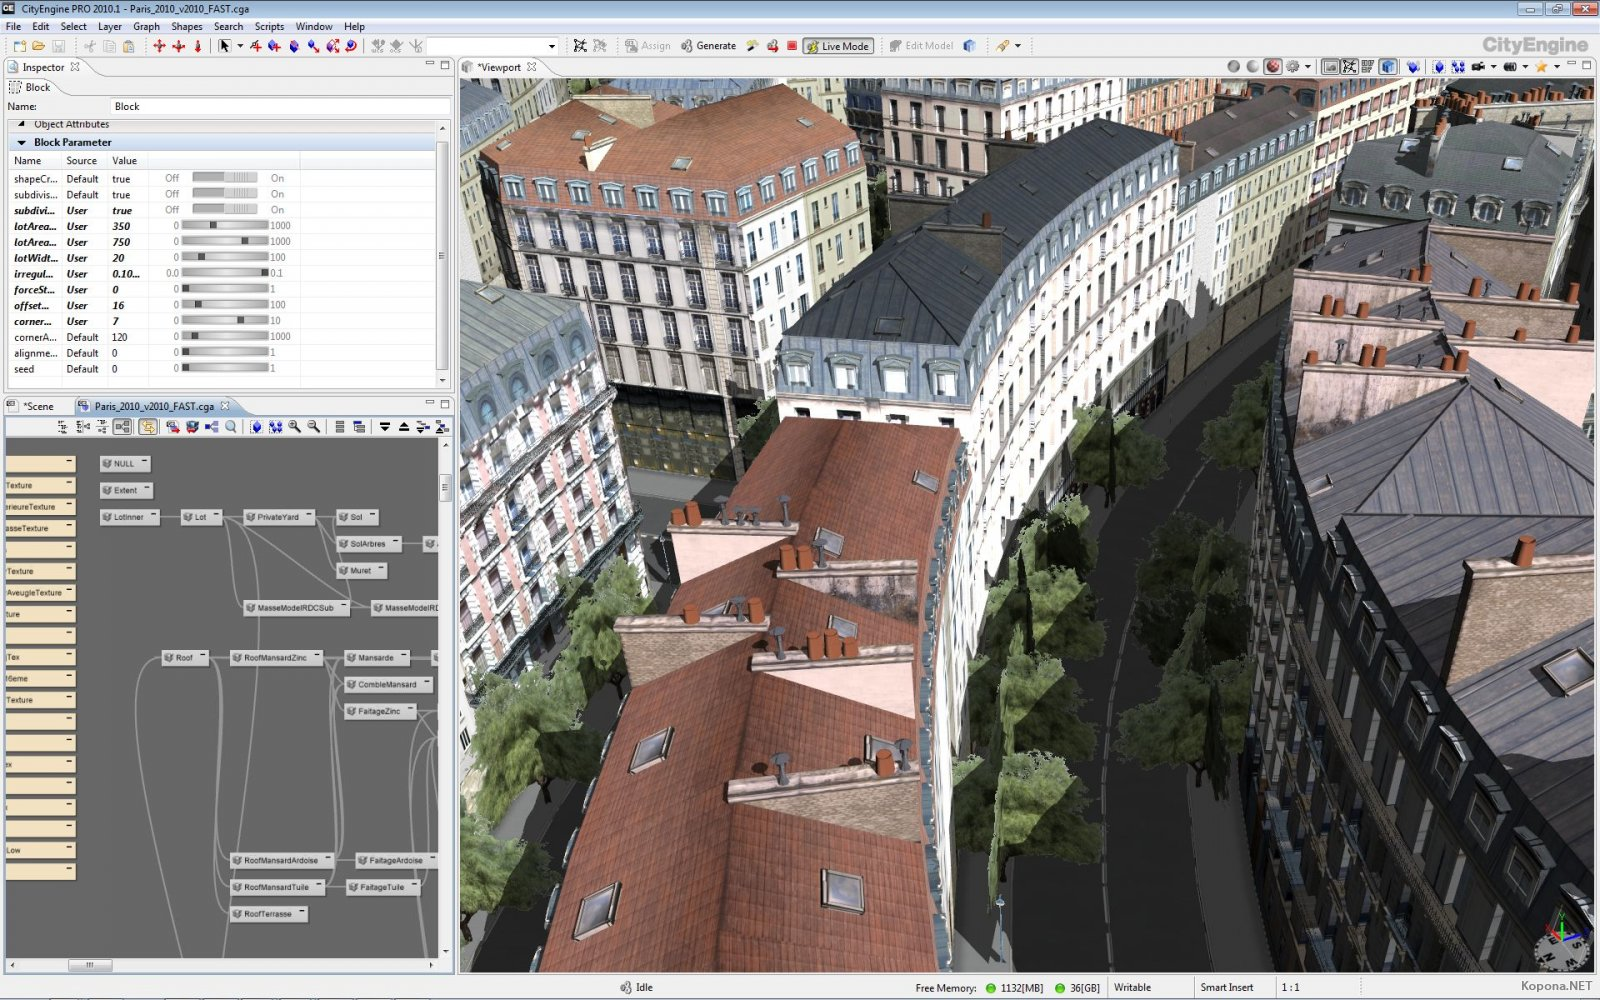
\includegraphics[width=\textwidth]{img/Procedural-Modeling-of-Cities/interface.jpg}
  \caption{City Engine Interface}
  \label{fig:CEinterface}
\end{figure}

\subsubsection{RoadNetwork} % (fold)
\label{ssub:roadnetwork1}


The first part to procedurally generate a city is to create a road network to become a backbone of the city and provide an overall structure. For that, CityEngine receives as input maps such as land-water boundaries and population
density. From that input a network of highways is created to connect the areas off high density population, and small roads connect to the highways.
This growth process continues until the average area of each lot is the desired one. The system have a default value, but it can be set by the user to a different one.

To implement this growth process, it uses an L-System (Section~\ref{ssub:l_systems}) that computes the road network.


\begin{figure}[htbp]
  \centering
  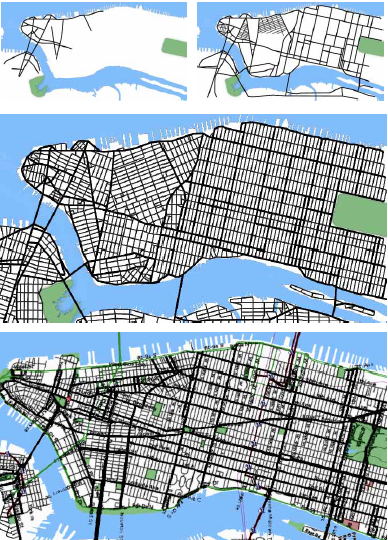
\includegraphics[width=0.5\textwidth]{img/Procedural-Modeling-of-Cities/Capturar.png}
  \caption{Road Map growth}
  \label{fig:city}
\end{figure}

The Figure~\ref{fig:city} shows the evolution of this process in a map of Manhattan. The first two pictures on the top shows the process in different phases during the process, the picture in the middle is the result of the process and the bottom line is the real map of Manhattan for comparison.

% subsubsection roadnetwork (end)Road Network

\subsubsection{Buildings} % (fold)
\label{ssub:buildings1}

To implement the generation of buildings, CGA was created, which is a shape grammar(Section~\ref{ssub:shape_grammars}) that was introduced in \cite{Parish2001}. It is defined as ``a novel shape grammar for the procedural modelling of CG architecture, produces building shells with high visual quality and geometric detail." To do so, this grammar uses a group of well defined production rules.

This tool allows the user to model buildings with an high control and in different ways. It can be done by text, writing production rules from a shape grammar or with a visual language similar Grasshopper 3D, that is nice for simple models but it is hard to work with more complex models, for instance, Figure~\ref{fig:CEinterface} shows a set of rules (bottom left), that is relatively small but is already difficult to follow the connections between rules.

\paragraph{Mass Modeling} % (fold)
\label{par:mass_modeling}
To model a building the first step is to create a mass model of the entire building by assembling basic shapes. With scaling, translation rotation and split applied to basic shapes namely I, L, H, U and T as shown in the Figure~\ref{fig:basic_shapes}.

\begin{figure}[htbp]
  \centering
  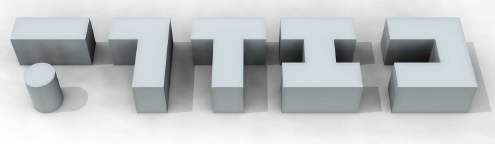
\includegraphics[width=0.95\textwidth]{img/Procedural-Modeling-of-Cities/MassModeling2.png}
  \caption{Basic shapes}
  \label{fig:basic_shapes}
\end{figure}

% paragraph mass_modeling (end)

The next step is to add the roof, from a set of basic roof shapes or general L-Systems.

After that, with the application of the grammar rules in the created mass, it is possible to create complexity to the level that is desired, being able to produce highly complex buildings like the one in Figure~\ref{fig:CEnewbuilding}.


\begin{figure}[htbp]
  \centering
  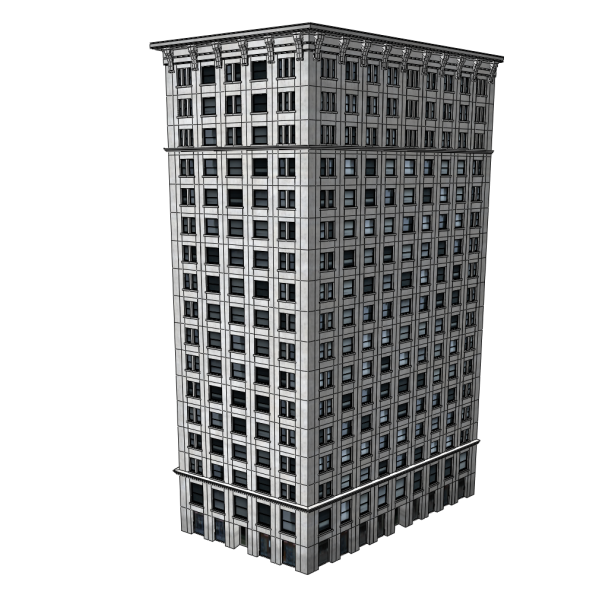
\includegraphics[width=0.8\textwidth]{img/Procedural-Modeling-of-Cities/building2.png}
  \caption{Complex building modeled with CGA}
  \label{fig:CEnewbuilding}
\end{figure}

% subsubsection buildings (end)

\subsubsection{Cities} % (fold)
\label{ssub:Cities1}

The result can be a city like Figure~\ref{fig:bigCity}, with approximately 26000 buildings.

\begin{figure}[htbp]
  \centering
  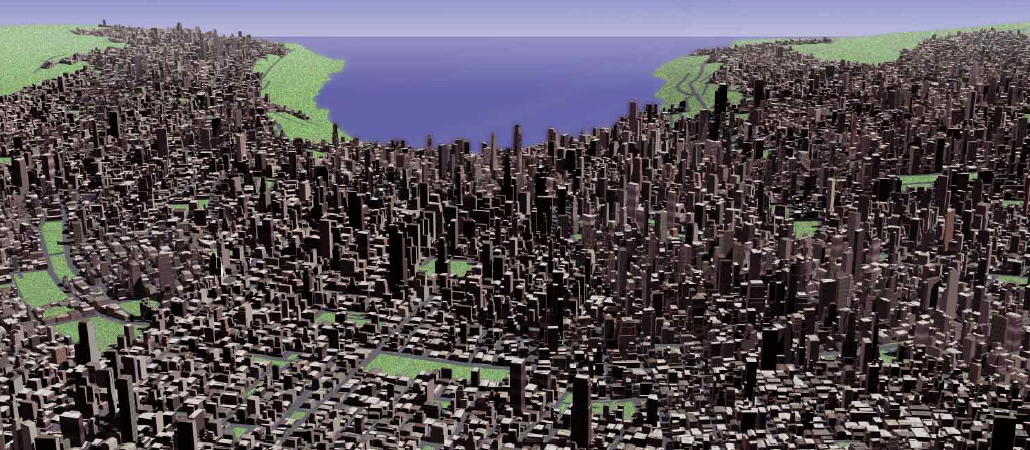
\includegraphics[width=0.95\textwidth]{img/Procedural-Modeling-of-Cities/City.png}
  \caption{City with approximately 26000 buildings.}
  \label{fig:bigCity}
\end{figure}

City Engine outputs can be imported by Maya\footnote{\url{http://www.autodesk.com/products/maya/overview}}, to achieve better results. Like the Figure~\ref{fig:cityMaya}, that represents a ‘virtual’ Manhattan.

\begin{figure}[htbp]
  \centering
  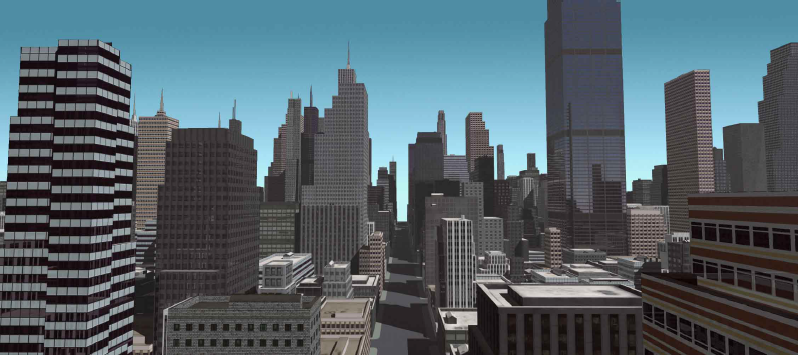
\includegraphics[width=0.95\textwidth]{img/Procedural-Modeling-of-Cities/City_Maya.png}
  \caption{City rendered with Maya.}
  \label{fig:cityMaya}
\end{figure}

% subsubsection subsubsection_name (end)
